\documentclass[11pt]{report}

\usepackage[margin=1in]{geometry} 
\usepackage{amsmath,amsthm,amssymb,amsfonts}

\usepackage[utf8]{inputenc}
\usepackage[T1]{fontenc}
\usepackage[spanish]{babel}

\usepackage{mathpazo,euler}
\usepackage{mathrsfs}
\usepackage{enumitem}
\usepackage{microtype}
\usepackage{tocbibind}
\usepackage[
    %textcolor=red,
    linecolor=color,
    bordercolor=color,
    backgroundcolor=white,
]{todonotes}
\usepackage{titlesec}

\usepackage{thmtools,xcolor}
\usepackage{fancyhdr}
\pagestyle{fancy}
\usepackage[misc]{ifsym}
\usepackage{tcolorbox}
\tcbuselibrary{theorems}

\usepackage{tikz}
\usepackage{tikz-cd}
\usetikzlibrary{arrows}
\usetikzlibrary{matrix}

\definecolor{color}{RGB}{34, 87, 46}
\addto\captionsspanish{\renewcommand{\chaptername}{Parte}}
\renewcommand\qedsymbol{$\paint{\blacklozenge}$}
\declaretheoremstyle[
  spaceabove = 6pt,
  spacebelow = 6pt,
  headfont=\color{color}\normalfont\bfseries,
  notefont=\color{color}\normalfont\bfseries
]{colored}
\theoremstyle{colored}

\newtheorem{definition}{Definición}[section]
\newtheorem{theorem}{Teorema}[section]
\newtheorem*{theorem*}{Teorema}
\newtheorem{proposition}{Proposición}[section]
\newtheorem{corollary}{Corolario}[section]
\newtheorem{lemma}{Lema}[section]
\newtheorem{remark}{Observación}[section]
\newtheorem{example}{Ejemplo}[section]
\newtheorem{exercise}{Ejercicio}[section]

\usepackage{hyperref}
\hypersetup{
    colorlinks,
    citecolor=color,
    filecolor=color,
    linkcolor=color,
    urlcolor=color,
}

\newcommand{\N}{\mathbb{N}}
\newcommand{\Z}{\mathbb{Z}}
\newcommand{\Q}{\mathbb{Q}}
\newcommand{\R}{\mathbb{R}}
\newcommand{\C}{\mathbb{C}}
\newcommand{\M}[2]{\mathsf{M}_{#1}#2}
\newcommand{\im}{\operatorname{im}}
\newcommand{\id}{\operatorname{id}}
\newcommand{\eps}{\varepsilon}
\newcommand{\nat}[1]{[\![#1]\!]}
\newcommand{\ord}[1]{\nat{#1}}
\newcommand{\natzero}[1]{\nat{#1}_0}
\newcommand{\ol}{\overline}
\newcommand{\tint}[1]{\stackrel{o}{#1}}
\newcommand*{\dt}[1]{\accentset{\mbox{\large\bfseries .}}{#1}}
\newcommand{\cat}[1]{\mathsf{#1}}
\newcommand{\sk}{\mathsf{sk}}
\renewcommand{\ss}[1]{\Delta^{#1}}
\newcommand{\bss}[1]{\partial \ss{n}}
\newcommand{\horn}[2]{\Lambda^{#1}_{#2}}
\newcommand{\ordcat}{\boldsymbol{\Delta}}
\newcommand{\catlim}[2]{\underset{#1}{\operatorname{lim}}#2}
\newcommand{\catcolim}[2]{\underset{#1}{\operatorname{colim}}#2}
\newcommand{\homcomplex}{\mathbf{Hom}}

\newcommand{\guill}[1]{«#1»}

\newcommand{\paint}[1]{\color{color}{#1}}
\newcommand{\tpaint}[1]{\paint{\textbf{#1}}}
\newcommand{\paintline}{\begin{center}
$\paint{
\rule{400pt}{0.5pt}
}$
\vspace{10pt}
\end{center}}

%-----------------------

\title{
\scshape\Huge{Topología Algebraica}
\\
\vspace{3pt}
\Large{Primer Cuatrimestre -- 2019}
\\
\vspace{0.5pt}
\Large{Examen Final}
\\
\vspace{80pt}
{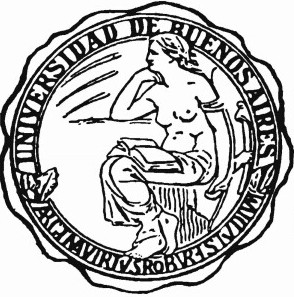
\includegraphics[height=5cm]{uba2.jpg}}
\vspace{80pt}
}
\author{\Large Guido Arnone}
\date{}
\lhead{Guido Arnone}
\rhead{Examen Final}

\begin{document}

\maketitle
\renewcommand{\contentsname}{Índice}
\tableofcontents
\chapter{Conjuntos Simpliciales, Realización Geométrica y CW Aproximación}

\section{Preliminares}

Comenzamos definiendo la categoría de ordinales finitos, que será la base de todas las definiciones posteriores. Incluimos también algunos resultados categóricos que utilizaremos más adelante.

\subsection{La categoría de ordinales finitos}

\begin{definition} Se define la \textbf{categoría $\ordcat$ de ordinales finitos} como la categoría que tiene por objetos a los conjuntos ordenados $\ord{n} := \{0 < 1 < \cdots < n\}$ para cada $n \in \N_0$, y cuyas flechas son las funciones $f : \ord{n} \to \ord{m}$ que resultan morfismos de posets. Definimos además, para cada $\ord{n} \in \ordcat$ e $i \in \natzero{n}$, los mapas de \textbf{cocaras} 
\begin{align*}
d^i : \ord{n-&1} \to \ord{n}\\
&j \mapsto \begin{cases}
j &\text{si $j < i$}\\
j+1 &\text{si $j \geq i$}
\end{cases}
\end{align*}
y los mapas de \textbf{codegeneraciones}
\begin{align*}
s^i : \ord{n+&1} \to \ord{n}\\
&j \mapsto \begin{cases}
j &\text{si $j \leq i$}\\
j-1 &\text{si $j > i$}
\end{cases}
\end{align*}
\end{definition}

\begin{proposition} Los mapas de cocaras y codegeneraciones satisfacen las siguientes \textit{identidades cosimpliciales},
\[
\begin{cases}
d^jd^i = d^id^{j-1} &\text{si $i < j$}\\
s^jd^i = d^is^{j-1} &\text{si $i < j$}\\
s^jd^j = s^jd^{j+1} = 1\\
s^jd^i = d^{i-1}s^j &\text{si $i > j+1$}\\
s^js^i = s^is^{j+1} &\text{si $i \leq j$}\\
\end{cases}
\]
\qed \\
\end{proposition}

\begin{proposition} Toda flecha $\ord{n} \xrightarrow{f} \ord{m}$ en $\ordcat$ se puede escribir como una composición de mapas de cocaras y codegeneraciones. \\ \qed
\end{proposition}

\begin{remark} En vista de las dos proposiciones anteriores,  usando los mapas de cocaras y codegeneraciones y las identidades cosimpliciales se puede dar «una presentación de $\ordcat$ en términos de generadores y relaciones». A grandes rasgos, esto nos permitirá definir los objetos relacionados a $\ordcat$ únicamente a partir de los mapas de cocaras y codegeneraciones.
\end{remark}

\begin{remark} Podemos también pensar a $\ordcat$ como la subcategoría plena de los conjuntos simpliciales ordenados dada por $n$-símplices estándar. Como todo morfismo $\ss{k} \to \ss{l}$ es simplicial, esto equivale a dar funciones $\{0,\dots,k\} \to \{0,\dots,l\}$ que preservan el orden.
\end{remark}

\subsection{Límites, Colímites, Adjunciones y (co)unidades}

\begin{proposition}\label{(co)limites-lugar-a-lugar} Si $\cat{A}$ es una categoría pequeña, el funtor olvido $\cat{C}^\cat{A} \to \cat{C}^\cat{ob A}$ crea estrictamente todos los (co)límites que existen en $\cat{C}$ y estos se definen objeto por objeto, es decir, para cada $c \in \cat{C}$ la evaluación $ev_c : \cat{C}^\cat{A} \to \cat{C}$ preserva todos los (co)límites que existen en $\cat{C}$.
\end{proposition}
\begin{proof} Ver \cite{ct-context}, Proposition 3.3.9.
\end{proof}

\begin{proposition} \label{lema-adj-cuadrados} Sean $F : \mathscr{C}  \rightleftarrows \mathscr{D} : G$ dos funtores equipados con una familia de isomorfismos $\mathscr{D}(Fc,d) \simeq C(c,Gd)$ para cada $c \in \mathscr{C}$ y $d \in \mathscr{D}$. La naturadlidad de esta colección es equivalente a que para todo morfismo con dominio y codominio como se muestra a continuación
\begin{center}
\begin{tikzcd}
Fc \arrow{r}{f^\sharp}\arrow{d}[left]{Fh} &d\arrow{d}{k} \\
Fc' \arrow{r}[below]{g^\sharp} &d'
\end{tikzcd}
\quad$\leftrightsquigarrow$\quad
\begin{tikzcd}
c \arrow{r}{f^\flat}\arrow{d}[left]{h} &Gd\arrow{d}{Gk} \\
c' \arrow{r}[below]{g^\flat} &Gd'
\end{tikzcd}
\end{center}
se tenga que el cuadrado de la izquierda conmuta si y sólo si lo hace el de la derecha.
\end{proposition}
\begin{proof} Ver \cite{ct-context}, Lemma 4.1.3.
\end{proof}

\begin{proposition} Dada una adjunción $F \vdash G$, se tienen dos transformaciones naturales $\eps: GF \Rightarrow 1_{\mathscr{C}}$ y $\eta : FG \Rightarrow 1_{\mathscr{D}}$ llamadas counidad y unidad de la adjunción. Si $c \in \mathscr{C}$, la componente $\eta_c : c \to GFc$ está dada por la transposición de la flecha $1_{Fc} : Fc \to Fc$. Del mismo modo, dado $d \in \mathscr{D}$ se define la componente $\eps_d : FGd \to d$ como la transposición de $1_{Gd} : Gd \to Gd$.
\end{proposition}
\begin{proof} Ver \cite{ct-context}, Lemma 4.2.3.
\end{proof}

\begin{theorem} \label{rapl-lapc} Si se tiene una adjunción de la forma
\begin{center}
\begin{tikzcd}
    \cat{\mathscr{C}} \arrow[bend left=35]{rr}{F}
  & \rotatebox{90}{$\vdash$}
  & \cat{\mathscr{D}} \arrow[bend left=35]{ll}{G}
\end{tikzcd}
\end{center}
entonces $G$ preserva límites y $F$ preserva colímites.
\end{theorem}
\begin{proof} Ver \cite{ct-context}, Theorem 4.5.2 y Theorem 4.5.3.
\end{proof}


\section{Conjuntos Simpliciales}

Ahora sí, pasamos a definir los conjuntos simpliciales:

\begin{definition} Un \textbf{conjunto simplcial} es un funtor $X : \ordcat^{op} \to \cat{Set}$. Concretamente, éste consiste de 
\begin{itemize}
\item[(i)] una sucesión $X_0,X_1,X_2, \dots$ de conjuntos, y \item[(ii)] para cada $n \in \N_0$ e $i \in \natzero{n}$, funciones 
$d_i : X_n \to X_{n-1}$ y $s_i : X_n \to X_{n+1}$ llamadas mapas de caras y degeneraciones respectivamente, que satisfacen las siguientes \textit{identidades simpliciales}:
\[
\begin{cases}
d_id_j = d_{j-1}d_i &\text{si $i < j$}\\
d_is_j = s_{j-1}d_i &\text{si $i < j$}\\
d_js_j = d_{j+1}s_j = 1\\
d_is_j = s_jd_{i-1} &\text{si $i > j+1$}\\
s_is_j = s_{j+1}s_i &\text{si $i \leq j$}\\
\end{cases}
\] 
\end{itemize}
En ocasiones utilizaremos la palabra \guill{complejo} para referirnos a un conjunto simplicial, cuando no haya ambiguedad. Notamos $x \in X$ si $x \in X_n$ para algún $n \in \N_0$, y decimos que $x$ es un \textbf{$n$-símplex generalizado}\footnote{Cuando no sea necesario aclararlo, diremos simplemente que $x$ es un símplex de $X$.} de $X$.\\
\end{definition}

\begin{definition} Dados dos complejos simpliciales $X,Y : \ordcat^{op} \to \cat{Set}$, un \textbf{morfismo de conjuntos simpliciales} de $X$ a $Y$ es una transformación natural $f : X \to Y$. Concretamente, esto consiste en dar una familia de funciones $f_n : X_n \to Y_n$ tales que, para cada $0 \leq i \leq n$, los siguientes diagramas conmutan
\begin{center}
\begin{tikzpicture}
\matrix (m) [matrix of math nodes,row sep=3em,column sep=4em,minimum width=2em]
  {
     X_n & X_{n-1} & & X_n & X_{n+1}\\
     Y_n & Y_{n-1} & & Y_n & Y_{n+1}\\};
  \path[-stealth]
    (m-1-1) edge node [left] {$f_n$} (m-2-1)
    (m-1-4) edge node [left] {$f_n$} (m-2-4)
    (m-1-2) edge node [right] {$f_{n-1}$} (m-2-2)
    (m-1-5) edge node [right] {$f_{n+1}$} (m-2-5)
    (m-1-1) edge node [above] {$d_i$} (m-1-2)
    (m-2-1) edge node [below] {$d_i$} (m-2-2)
    (m-1-4) edge node [above] {$s_i$} (m-1-5)
    (m-2-4) edge node [below] {$s_i$} (m-2-5);
\end{tikzpicture} 
\end{center}

Es decir, un morfismo de conjuntos simpliciales consiste de una colección de aplicaciones que sea compatible con los mapas de caras y degeneraciones.
\end{definition}

\begin{remark} Los conjuntos simpliciales junto con los morfismos antes definidos forman una categoría\footnote{Esta es precisamente la categoría de prehaces de $\ordcat$.}, que notaremos $\cat{sSet}$.
\end{remark}

\subsection{Ejemplos}

\begin{example}[el $n$-símplex estándar] Para cada $n \in \N_0$ tenemos un conjunto simplicial dado por el funtor $\ordcat(-,\ord{n})$. Conrectamente, para cada $m \geq 0$ definimos los conjuntos
\[
\ss{n}_m := \ordcat(\ord{m},\ord{n}) = \{f : \ord{m} \to \ord{n} : \text{ $f$ es morfismo de posets } \}
\]
y los mapas de caras y degeneraciones están dados por
\[
(d^i)^* : f \in \ordcat(\ord{m},\ord{n}) \mapsto fd^i \in \ordcat(\ord{m-1},\ord{n})
\]
y
\[
(s^i)^* : f \in \ordcat(\ord{m},\ord{n}) \mapsto fs^i \in \ordcat(\ord{m+1},\ord{n}).
\]
Llamamos a este conjunto simplicial el \textbf{n-símplex estándar} y lo notamos $\ss{n}$.
\end{example}

Una vez más interpretando a $\ord{n}$ como el $n$-símplex combinatorio ordenado, su conjunto simplicial asociado consiste de «todas las formas posibles de incluir o colapsar un $m$-símplex estándar en $\nat{n}$».

Extendiendo esta interpretación tenemos el siguiente ejemplo,

\begin{example}[complejos simpliciales ordenados] Sea $K$ un complejo simplicial equipado con una relación de orden total para sus vértices $V = \{v_i\}_{i \in I}$. Notamos a cada $n$-símplex como una $n$-upla $[v_{i_0},\dots, v_{i_n}]$ con $v_k < v_{k+1}$ para cada $k$.

Asociaremos a $K$ un conjunto simplicial, agregando como en el caso de $\ss{n}$ la noción de \textit{símlpices degenerados}. Concretamente, para cada $n \in \N_0$ definimos
\[
K_n := \left\{[v_{i_0}, \dots, v_{i_n}] : \text{ $v_{i_k} \leq v_{i_{k+1}}$ para cada $k$, y $\{v_{i_k}\}_{k = 0}^n \in K$ }\right\}.
\]

En otras palabras, el conjunto $K_n$ consiste de $n$-uplas ordenadas de vértices que forman un símplex de $K$, pero permitiendo repetición. Definimos a su vez los mapas de caras y degeneraciones como
\[
d_k[v_{i_0}, \dots, v_{i_n}] := [v_{i_0},\dots,\widehat{v_{i_k}},\dots, v_{i_n}] \quad \text{y} \quad
s_k[v_{i_0}, \dots, v_{i_n}] := [v_{i_0},\dots,v_{i_k},v_{i_k}, \dots, v_{i_n}].
\]
\end{example}

\begin{remark} Un morfismo $f : K \to L$ de complejos simlpiciales ordenados induce a su vez un morfismo de conjuntos simpliciales dado por $f_n[v_{i_1}, \dots, v_{i_n}] := [f(v_{i_1}), \dots, f(v_{i_n})]$ para cada $n$-símplex $[v_{i_1}, \dots, v_{i_n}]$ (posiblemente degenerado) de $K$.

De forma similar, una función continua $f : X \to Y$ induce un morfismo $f_* : \mathcal{S}(X) \to \mathcal{S}(Y)$ entre conjuntos singulares vía la postcomposición. De hecho, 
\end{remark}

\begin{definition} Dado un $n$-śimplex estándar (como complejo simplicial), su \textbf{borde} es el complejo $\bss{n}$ dado por la unión de sus caras maximales y su $k$-ésimo \textbf{cuerno} es el subcomplejo $\horn{n}{k}$ de $\bss{n}$ que se obtiene quitando la $k$-ésima cara maximal de $\ss{n}$, para cierto $0 \leq k \leq n$. Decimos que $\horn{n}{k}$ es un cuerno \textit{interno} si $0 < k < n$, y \textit{externo} en caso contrario.
\end{definition}

Ahora sí, veamos un primer ejemplo topológico:

\begin{example} Sea $X$ un espacio topológico. Para cada $n \in \N_0$ definimos el conjunto
\[
\mathcal{S}(X)_n := \cat{Top}(|\ss{n}|,X)
\]
de todos los $n$-simplices singulares de $X$, y las aplicaciones 
\[
d_i : \mathcal{S}(X)_n \to \mathcal{S}(X)_{n-1}, \quad
s_i : \mathcal{S}(X)_n \to \mathcal{S}(X)_{n+1}
\]
que envían un $n$-símplex singular a la restricción $d_i\sigma$ a su $i$-ésima cara y al $(n+1)$-simplex singular $s_i\sigma$ que corresponde a colapsar $|\ss{n+1}|$ a $|\ss{n}|$ a través de $|s^i|$ y luego componer con $\sigma$.

Estos conforman el conjunto simplicial $\mathcal{S}(X)$ que se conoce como el \textbf{conjunto singular} de $X$.
\end{example}

\begin{definition} Dado un conjunto simplicial $X$, definimos su \textbf{complejo de Moore} como el complejo de cadenas
\[
\cdots \to \Z X_2 \xrightarrow{\partial} \Z X_1 \xrightarrow{\partial} \Z X_0,
\]
con $\Z X_n$ el grupo abeliano libre generado por el conjunto $X_n$ y 
\[
\partial = \sum_{i=1}^n(-1)^i d_i
\]
para cada $n \geq 0$.
\end{definition}

\begin{remark} La homología singular de un espacio topológico $X$ coincide con la homología del complejo de Moore de su conjunto singular. En general,
\end{remark}

\begin{definition} Sea $X$ un conjunto simplicial. Definimos su \textbf{homología} con coeficientes en $\Z$ como la homología del complejo de Moore asociado a $X$.
\end{definition}

\begin{example}[nervio de una categoría] Sea $\mathscr{C}$ una categoría localmente pequeña. Definimos el \textbf{nervio} de  $\mathscr{C}$ como el conjunto simplicial dado por los conjuntos
\begin{align*}
N(\mathscr{C})_n = \hom(\mathbf{n},\mathscr{C}) &= \{(f_1,\dots, f_k) : f_i \in \operatorname{mor} \mathscr{C}, \ \operatorname{cod} f_i = \operatorname{dom}f_{i+1}\}\\
& = \{x_0 \xrightarrow{f_1} x_1 \xrightarrow{f_2} \cdots \xrightarrow{f_n} x_n\}
\end{align*}
de $n$-uplas de morfismos componibles junto con los mapas 
\[
d_i(f_1, \dots, f_n) = (f_1, \dots,f_{i-1}, \ f_i \circ f_{i+1} \ ,\dots,f_n)
\]
y
\[
s_i(f_1, \dots, f_n) = (f_1, \dots, f_i, 1, f_{i+1},\dots,f_n),
\]
para cada $0 \leq i \leq n$. 

En particular, si $\mathscr{C} = BG$ es el grupoide asociado a un grupo $G$, entonces su nervio consiste de $n$-uplas de elementos de $G$ y los mapas de caras y degeneraciones están dados por
\[
d_i(g_1, \dots, g_n) = (g_1,\dots, g_{i-1},g_ig_{i+1},\dots,g_n), \quad s_i(g_1, \dots,g_n) = (g_1, \dots,g_i,1,g_{i+1},\dots,g_n).
\]
\end{example}

\begin{definition} El \textbf{funtor singular} $\mathcal{S} : \cat{Top} \to \cat{sSet}$ asigna a cada espacio su conjunto singular, y a cada función continua $f : X \to Y$ el morfismo simplicial $f_* : \mathcal{S}(X) \to \mathcal{S}(Y)$ dado por $(f_*)_n(\sigma) =  f \circ \sigma$ para cada $\sigma: |\ss{n}| \to X$.
\end{definition}

\begin{remark} Si $X$ es un conjunto simplicial, el conjunto $X_n$ está determinado por los morfismos de conjuntos simpliciales de $\ss{n}$ a $X$. 

Concretamente, por el lema de Yoneda tenemos una biyección natural
\[
\hom_{\cat{sSet}}(\ss{n},X) \simeq X_n
\]

que a cada elemento $x \in X_n$ le asigna un morfismo de conjuntos simpliciales $\iota_x : \ss{n} \to X$ que satisface $\iota_x(1_{\ord{n}}) = x$. 

Esto se corresponde con la intuición que proveen los ejemplos anteriores, en los que los $n$-símplices de un conjunto simplicial son alguna «manifestación» de el $n$-símplex estándar: como la cara de un $m$-símplex de dimensión mayor, como un $m$-símplex de dimensión menor que represente un colapso del mismo, o como el $n$-símplex singular de un espacio topológico.\\
\end{remark}

\subsection{Símplices Degenerados, Puntos Interiores y Esqueletos}

\begin{definition} Sea $X$ un conjunto simplicial. Un $n$-simplex $x \in X_n$ se dice \textbf{degenerado} si existe $y \in X_{n-1}$ tal que $s_i(y) = x$ para algún $i \in \natzero{n}$. En caso contrario, decimos que $x$ es \textbf{no degenerado}. 

Notamos $NX_n := \{x \in X_n : \text{ $x$ es no degenerado}\}$ y $NX_{\leq n} = \bigcup_{0 \leq k \leq n}NX_k$ para cada $n \in \N_0$. Definimos también el conjunto $NX := \bigcup_{n \in \N_0}NX_n$ de todos los símplices no degenerados.
\end{definition}

\begin{proposition} Sea $X$ un conjunto simplicial. Si $x \in X$ es un símplex degenerado, entonces existe un único símplex no degenerado $y \in X$ tal que $x = s_{i_1} \cdots s_{i_k}y$.
\end{proposition}
\begin{proof} Como $x$ es degenerado, sabemos que existe $x_1 \in X$ y un mapa de degeneración $s_{i_1}$ tal que $x = s_{i_1}(x_1)$. 

Procediendo inductivamente\footnote{Notemos que el proceso termina pues cada símplex que tomamos tiene una dimensión menos, y un $0$-símplex nunca es degenerado.}, obtenemos una sucesión de mapas de degeneración $s_{i_1},\dots, s_{i_k}$ y un símplex no degenerado $y \in X$ tal que
\[
x = s_{i_1} \cdots s_{i_k}(y).
\]

Para terminar, veamos la unicidad. Supongamos que existen mapas de degeneraciones $s_{j_1}, \dots, s_{j_l}$ y un símplex $z \in X$ tales que
\[
s_{i_1} \cdots s_{i_k}(y) = x = s_{j_1} \cdots s_{j_l}(z).
\]
Componiendo a derecha por $d_{i_k} \cdots d_{i_1}$, es
\[
y = d_{i_k} \cdots d_{i_1}s_{j_1} \cdots s_{j_l}(z).
\]

Usando las identidades simpliciales, podemos «reordenar» los mapas de forma que existen $s$ y $d$, composiciones de mapas de caras y degeneraciones respectivamente, que satisfacen
\[
y = sd(z).
\]
Como $y$ es no degenerado, debe ser $s = 1$ y por lo tanto $y = dz$ es una cara de $z$. Por simetría, vemos también que $z$ es una cara de $y$. En particular, los símplices $z$ e $y$ deben tener la misma dimensión, por lo que debe ser $d = 1$ y $z = y$. 
\end{proof}

\begin{definition} Sea $k \in \N_0$. Un punto $p \in |\ss{k}|$ del $k$-símplex topólogico se dice \textbf{interior} si no existe un mapa de cocara $d^i : \ss{k-1} \to \ss{k}$ y $q \in |\ss{k-1}|$ tal que $|d^i|(q) = p$.
\end{definition}

\begin{proposition} Sea $k \in \N_0$ y $p \in |\ss{k}|$. Si $p$ es interior, existen únicos $l \in \N_0$, $q \in |\ss{l}|$ y $d^{i_1}, \dots, d^{i_s}$ mapas de cocara tales que $p = |d^{i_1} \cdots d^{i_s}|(q)$.
\end{proposition}
\begin{proof} Como $p$ es interior, existe un mapa de cocara $d^{i_1}$ y $q_1 \in |\Delta^{k-1}|$ tal que $d^{i_1}q_1 = p$. Procedemos inductivamente obtenemos la existencia. 

Ahora, supongamos que $q \in |\ss{k}|,q'\in|\ss{k'}|$ son tales que existen mapas de cocara $d^{i_1}, \dots, d^{i_r},d^{j_1}, \dots, d^{j_s}$ con $|d^{i_1}, \dots, d^{i_s}|(q) = |d^{j_1}, \dots, d^{j_s}|(q')$. Usando las identidades cosimpliciales existen funciones $s, \ d$ que son composiciones de codegeneraciones y cocaras respectivamente, y satisfacen
\[
q = |ds|(q').
\]
Como $q$ es interior, debe ser $|d| = 1$ y entonces $q'$ se colapsa a $q$. Por simetría tenemos entonces que ambos puntos se colapsan el uno al otro: esto implica $s = 1$ y $q  = q'$.
\end{proof}

\begin{corollary} Si $p \in |\ss{k+1}|$ es interior, y $s^j$ es un mapa de codegeneración, entonces $s_j(p)$ es interior. 
\end{corollary}
\begin{proof} Notemos que para todo $\sum_{i=1}^{n-1}\alpha_ ie_i \in |\ss{n-1}|$ y mapa de cocara $d^i$, es 
\[
d^iz= \sum_{j=1}^{i-1}\alpha_j e_j + \sum_{j = i+1}^{n}\alpha_{j-1} e_j.
\]
Por lo tanto, un punto interior debe tener todas sus coordenadas no nulas. En consecuencia el punto $p = \sum_{j=1}^{k+1}\alpha_je_j \in |\ss{k+1}|$ debe tener todas sus coordenadas no nulas. Como es
\[
s^j(p) = \sum_{j < i}\alpha_j e_j + (\alpha_i+\alpha_{i+1})e_i + \sum_{j > i+1}^k \alpha_{j}e_{j-1}
\]
que una vez más tiene todas sus coordenadas no nulas, debe ser entonces un punto interior.
\end{proof}

\begin{definition} Sea $X$ un conjunto simplicial. Un \textbf{subconjunto simplicial} o subcomplejo de $X$ es un conjunto simplicial $K$ junto con un morfismo simplicial $K \hookrightarrow X$ que en cada nivel es una inclusión de conjuntos $K_n \hookrightarrow X_n$.
\end{definition}

\begin{definition} Sea $X$ un conjunto simplicial y $n \in \N_0$. Definimos el $n$-esqueleto $\sk_n X$ de $X$ como el menor subcomplejo de $X$ que tiene a los $j$-símplices de $X$ para cada $j \in \natzero{n}$. Es decir, es el complejo
\[
(\sk_nX)_j = \begin{cases}
X_j &\text{si $j \leq n$}\\
\{x \in X_j : x = s_{i_1} \cdots s_{i_{j-n}}y \text{ con } y \in X_n\} &\text{si $j > n$}
\end{cases}
\]
junto con las restricciones de los mapas de caras y degeneraciones de $X$. Notemos que si $k < l$ por construcción es $(\sk_k X)_j \subset (\sk_l X)_j$ para todo $j \geq 0$, por lo que tenemos las siguientes \guill{inclusiones} de subcomplejos,
\[
\sk_0X \subset \sk_1X \subset \sk_2X \subset \cdots \subset \sk_nX \subset \cdots
\]
\todo{Probar que $X \simeq \operatorname{colim} \sk_nX$}
\end{definition}

\subsection{Productos, Coproductos, Pushouts}

\begin{definition} Sean $X$ e $Y$ dos conjuntos simpliciales. Se define su \textbf{producto} como el conjunto simplicial dado por los conjutos $X_n \times Y_n$ y cuyos mapas de caras y degeneraciones son las funciones producto $d_i = d_i^X \times d_i^Y, s_i = s_i^X \times s_i^Y$ de los mapas de caras y degeneraciones de cada conjunto simplicial. Lo notamos $X \times Y$, pues es el objeto producto en $\cat{sSet}$.
\end{definition}

\begin{definition} Sean $X$ e $Y$ dos conjuntos simpliciales. Se define su \textbf{coproducto} como el conjunto simplicial dado por los conjuntos $X_n \sqcup Y_n$ y mapas de caras y degeneraciones dados por la unión disjunta $d_i = d_i^X \sqcup d_i^Y, s_i = s_i^X \sqcup s_i^Y$ de los mapas de cada espacio. Lo notamos $X \sqcup Y$ ya que es el objeto coproducto en $\cat{sSet}$.
\end{definition}

\begin{remark} Por la Proposición \ref{(co)limites-lugar-a-lugar} y usando que $\cat{Set}$ es cocompleta\footnote{Una categoría $\cat{C}$ es (co)completa si existe el (co)límite de todo diagrama $\cat{J} \to \cat{C}$.}, los pushouts en $\cat{sSet}$ se pueden construir \guill{nivel a nivel}, es decir, a partir del pushout de los conjuntos en el lugar $n$ de cada complejo.
\end{remark}

\begin{proposition}\label{sk-pushout} Si $X$ es un conjunto simplicial y $n \in \N$, entonces el siguiente diagrama es un pushout
\begin{center}
\begin{tikzcd}
\coprod_{n \in NX_n} \partial \ss{n} \arrow{d}\arrow{r}& \sk_{n-1}X\arrow{d}\\
\coprod_{n \in NX_n} \ss{n} \arrow{r}& \sk_nX\\
\end{tikzcd}
\end{center}
es un puhsout.
\end{proposition}
\begin{proof}asd
\todo{¡HACER!}
\end{proof}

\subsection{Complejos de Funciones y Ley Exponencial}

Para definir las nociones siguientes, necesitamos primero definir complejos de funciones y probar una versión simplicial de la ley exponencial.

\begin{definition} Sean $X$ e $Y$ conjuntos simpliciales. Definimos el \textbf{complejo de funciones} $\homcomplex(X,Y)$ dado por
\[
\homcomplex(X,Y)_n := \hom_{\cat{sSet}}(X \times \ss{n},Y)
\]
para cada $n \in \N_0$ y 
\begin{align*}
\theta^* : \homcomplex(X,&Y)_m \to \homcomplex(X,Y)_n \\
&f \longmapsto f \circ (1_X \times \theta)
\end{align*}
para cada $\ord{n} \xrightarrow{\theta} \ord{m}$.
\end{definition}

\begin{definition} Dados $X$ e $Y$ conjuntos simpliciales, se define la \textbf{función evaluación}
\[
ev : X \times \homcomplex(X,Y) \to Y.
\]
dada por $ev_n(x,f) = f(x,1_n)$. Esta resulta un morfismo simplicial que natural en ambas variables.
\end{definition}

\begin{theorem}[Ley Exponencial] Si $K,X$ e $Y$ son conjuntos simpliciales, la aplicación
\begin{align*}
ev_* : \hom_{\cat{sSet}}(K,\homcomplex(X,Y&)) \to \hom_{\cat{sSet}}(X \times K,Y)\\
&g \longmapsto ev \circ (1_X \times g)
\end{align*}
está bien definida y es biyectiva. Más aún, esta resulta natural en las tres variables.
\end{theorem}
\begin{proof} Damos solo la aplicación inversa, los demás detalles se pueden ver en \cite{GJ}, Chapter 1, Section 5 y en \cite{M}, Chapter 1, \S 6. Recordemos que un elemento $x \in X_n$ se corresponde con una flecha $\iota_x : \ss{n} \to X$. La inversa de $ev_*$ envía entonces $f : X \times K \to Y$ a $x \mapsto f \circ (1_X \times \iota_x)$.
\end{proof}

\section{Realización Geométrica}

Durante la materia vimos como a partir de un complejo simplicial $K$ podemos construir un espacio topológico $|K|$, la realización geométrica de $K$. Siguiendo esta idea, queremos extender esta noción al contexto de los conjuntos simpliciales.

\begin{definition} Sea $X$ un conjunto simplicial. Dotando a cada conjunto $X_n$ de la topología discreta, definimos la \textbf{realización geométrica} de $X$ como el espacio
\[
|X| = \left(\coprod_{n \geq 0}X_n \times |\ss{n}|\right)\Big/\sim
\]
donde identificamos a los puntos $(x,|d^i|(p)) \sim (d_i(x),p)$ y $(x,|s^i|(p)) \sim (s_i(x),p)$.
\end{definition}

Esto formaliza la intuición anterior: para cada $x \in X_n$ construimos una copia del $n$-símplex estándar y los pegamos en función de si son caras o colapsos unos de otros.

Además, como veremos en breve esta asignación es funtorial, teniéndose así un análogo a la realización geométrica para complejos simpliciales. Más aún, estas nociones coindicen cuando $X$ es el conjunto simplicial asociado a un complejo simplicial ordenado.

\subsection{Ejemplos}

\begin{proposition} La realización geométrica del $n$-símplex estándar $\ss{n} :\ordcat^{op} \to \cat{Set}$ es homeomorfa a la realización geométrica del $n$-símplex estándar como complejo simplicial.
\end{proposition}
\begin{proof} Para evitar ambiguedades, en toda la demostración notaremos $|\ss{n}|$ exclusivamente para referirnos a la realización geométrica del $n$-símplex como complejo simplicial. Por otro lado, notaremos $|\ordcat(-,n)|$.

Para cada $k \in \N_0$ tenemos una aplicación
\[
(f,x) \in \ordcat(k,n) \times |\Delta^k| \to |f|(x) \in |\Delta^n|,
\]
que resulta continua pues cada espacio $\ordcat(k,n)$ es discreto.

Ésta familia de funciones induce un morfismo en el coproducto que pasa al cociente por las identificaciones de la realización geométrica, pues si $g$ es un mapa de cocara o codegeneración, entonces
\[
r(g^*(f),x) = |fg|(x) = r(f,|g|(x)).
\]
Se tiene entonces una función continua $r : [(f,x)] \in |\ordcat(-,n)| \to |f|(x) \in |\Delta^n|$. 

Por otro lado, podemos considerar la inclusión $i : |\ss{n}| \to |\ordcat(-,n)|$ dada por la composición
\[
|\ss{n}| \xrightarrow{\simeq} \{id\} \times |\ss{n}| \hookrightarrow |\ordcat(-,n)|,
\]
que satisface $ri = 1$ pues
\[
ri(x) = [(id,x)] = |id|(x) = x
\]
para todo $x \in |\ss{n}|$. En particular sabemos que $i$ es inyectiva. Por lo tanto, para terminar basta ver que $i$ es sobreyectiva, en cuyo caso es un homeomorfismo con inversa $f$.

Equivalentemente, resta ver que todo elemento $[(f,x)]$ está relacionado con un punto de la forma $(id,y)$ para cierto $y \in |\ss{n}|$. En efecto, sea $(f,x) \in |\ordcat(-,n)|$ con $f : \ord{k} \to \ord{n}$ un morfismo de posets y $x \in |\ss{k}|$. Sabemos entonces que existen mapas de cocara o codegeneración $f_1, \dots, f_n$ tales que $f = f_1 \cdots f_n$. En consecuencia es
\begin{align*}
[(f,x)] &= [(f_1 \cdots f_n, x)] = [(f_n^* \circ \cdots \circ f_1^*(id), x)]\\ &= [(id,|f_1 \cdots f_n|(x))] = [(id, |f|(x))],
\end{align*}
lo que concluye la demostración.
\end{proof}

\begin{proposition} Si $K$ es un complejo simplicial ordenado, entonces sus realizaciones geométricas como conjunto y complejo simplicial coinciden.
\end{proposition}
\begin{proof} Notemos $\mathfrak{K}$ a la realización geométrica de $K$ como conjunto simplicial y $|K|$ a la realización geométrica como complejo simplicial. Para cada símplex generalizado $x  = [v_{i_1}\cdots v_{i_k}]$, notamos $\Delta_x := \{v_{i_1}, \dots, v_{i_k}\}$. De la misma forma, notaremos $[\sigma]$ al símplex ordenado que se corresponde con $\sigma \in K$.

Ahora, tenemos una flecha $|\ss{k}| \to |\Delta_x|$ vía el morfismo de posets que envía a cada $s \in \ord{k}$ a $v_{i_s}$, lo que induce una función continua  $f_x : \{x\} \times |\Delta^k| \to |\Delta_x|$ para cada $x\in X$. A través de la inclusión $|\Delta_x| \hookrightarrow |K|$ obtenemos finalmente funciones continuas $ \{x\} \times |\ss{k}| \to |K|$ para cada $x \in X$. Por un cálculo directo, siempre se tiene $f_{d_i(x)}(p)  = f_x(|d^i|(p))$ y $f_{s_i(x)}(p) = f_x(|s^i|(p))$, así que estas inducen una aplicación continua
\[
f: \mathfrak{K} \to |K|.
\]

Por otro lado, tenemos una función $g : |K| \to \mathfrak{K}$ que envía la combinación convexa (ordenada, con escalares no nulos) $\sum_{i=1}^k a_iv_{i_k}$ a la clase del elemento $([v_{i_1}, \dots, v_{i_k}] ,a_1e_1 + \dots + a_ke_k)$.

La continuidad de $g$ se desprende de que el diagrama
\begin{center}
\begin{tikzcd}
\text{$|K|$} \arrow{r}{g} &\mathfrak{K}\\
\text{$|\sigma|$} \arrow[hook]{u} \arrow{r}{\equiv} & \text{$\{[\sigma]\} \times |\ss{k}|$} \arrow[hook]{u}
\end{tikzcd}
\end{center}
es conmutativo para cada $k$-símplex $\sigma \in K$ y $|K|$ tiene la topología final con respecto a sus símplices. 

Para terminar, veamos que $f$ y $g$ son inversas: por construcción, para cada símplex $\sigma \in K$ se tiene que $f_{[\sigma]}g|_{|\sigma|} = 1$, así que ya sabemos que $fg = 1$. Por otro lado, si $x \in X$ es no degenerado entonces es $[\Delta_x] = x$ y  $g|_{|\Delta_x|}f_x = 1$. Como todo punto de $\mathfrak{K}$ es equivalente a la clase de uno cuyo símplex generalizado es no degenerado, obtenemos finalmente que $gf = 1$.
\end{proof}

Vemos así que la construcción que dimos efectivamente generaliza a la de realización geométrica para complejos simpliciales: tiene sentido preguntarse entonces, ¿qué sucede cuando $X$ no necesariamente viene inducido por un complejo simplicial? Veremos más adelante que el espacio topológico $|X|$ siempre es un CW-complejo.

\begin{definition} Sea $X$ un conjunto simplicial. Un punto $(x,p) \in \coprod_{n \geq 0} X_n \times |\ss{n}|$ se dice \textbf{no degenerado} si $p$ es interior y $x$ no degenerado.
\end{definition}

\begin{lemma}\label{uniq-pt-nodeg} Sea $X$ un conjunto simplicial. Si $(x,p) \in \coprod_{n \geq 0} X_n \times |\ss{n}|$, entonces existe un único punto no degerado $(y,q)$ relacionado con $(x,p)$.
\end{lemma}
\begin{proof} Para cada símplex $x \in X$, sabemos que existe un único símplex no degenerado $y \in X$ y $s = X(\sigma)$ una composición de mapas de degeneración tales que $s(y) = x$. Del mismo modo, existe un único punto $q$ de un símplex topológico y una composición de mapas de cocaras $\delta$ tales que $p = \delta(q)$. Notando $\lambda(x,p) := (y,\sigma p)$ y $\rho(x,p) := (X(\delta)(x),q)$, tenemos definidas dos aplicaciones
\[
\lambda, \rho : \coprod_{n \geq 0} X_n \times |\ss{n}| \to \coprod_{n \geq 0} X_n \times |\ss{n}|
\] 

Más aún, la imagen de $\lambda$ consiste de puntos cuyo símplice de $X$ es no degenerado, y por otro lado la imagen de lambda consiste de pares cuyo elemento del símplex topológico es interior. Por lo tanto, la composición
\[
\Phi := \lambda \circ \rho : \coprod_{n \geq 0} X_n \times |\ss{n}| \to \coprod_{n \geq 0} X_n \times |\ss{n}|
\]
envía cada punto a uno relacionado que es no degenerado, lo que prueba la existencia.

Notemos además que $\Phi$ deja fijos a los puntos no degenerados, así que para ver la unicidad resta probar que puntos relacionados tienen la misma imagen por $\Phi$. De hecho, alcanza probar que  $\Phi(X(d)x,p) = \Phi(x,|d|p)$ y $\Phi(X(s)x,|s|p)$ para cada mapa de cocara $d$ y codegeneración $s$. 

Tomemos un punto $(x,p)$ con $p = |\delta|q$ y $q$ interior. Se tiene entonces que
\[
\rho(X(d)x,p) = \rho(X(d),|\delta|q) = (X(\delta)X(d)x,q) = (X(d\delta)x,q) = \rho(x,|d\delta|q) = \rho(x,|d|p),
\]
para cada mapa $d$ de cocara. En particular debe ser $\Phi(X(d)x,p) = \Phi(x,|d|p)$. 

Si ahora $s$ es un mapa de degeneración, podemos escribir $s\delta = \delta's'$ y $X(\delta')x = X(\sigma)z$ y cierta composición de mapas de cocara $\delta'$ y codegeneración $s',\sigma$, con $z$ no degenerado. Con esta notación es
\[
X(\delta)X(s)x = X(s\delta)x = X(\delta's')x = X(s')X(\delta')x = X(s')X(\sigma)z = X(\sigma s')z.
\]
lo que finalmente dice que
\begin{align*}
\Phi(X(s)x,p) &= \lambda(X(\delta)X(s)x,q) = \lambda(X(\sigma s')z,q) = (z,|\sigma s'|q)\\
&= \lambda(X(\sigma)z,|s'|q) = \lambda(X(\delta')x,|s'|q) = \lambda\rho(x,|\delta's'|q)\\
&= \Phi(x,|s\delta|q) = \Phi(x,|s|p).
\end{align*}
\end{proof}

\subsection{Funtorialidad y adjunción entre la realización geométrica y el funtor singular}

\begin{definition} Sea $X$ un conjunto simplicial. Su \textbf{categoría de símplices} es la categoría coma $\Delta \downarrow X$, donde $\Delta: \ordcat \to \cat{Set}^{\ordcat^{op}}$ es el embedding de Yoneda de $\ordcat$ y $X : \ordcat \to \cat{Set}^{\ordcat^{op}}$ es el funtor que vale constantemente $X$. Concretamente, los objetos de $\Delta \downarrow X$ son \textit{símplices} de $X$, entendidos como morfismos simpliciales $\ss{n} \to X$, y las flechas son morfismos $\theta : \ord{n} \to \ord{m}$ de posets tales que el diagrama
\begin{center}
\begin{tikzpicture}
\matrix (m) [matrix of math nodes,row sep=3em,column sep=4em,minimum width=2em]
  {
     \ss{n}& &\\
     & & X\\
     \ss{m} & &\\};
  \path[-stealth]
    (m-1-1) edge node [above] {$\sigma$} (m-2-3)
    (m-1-1) edge node [left] {$\theta_*$} (m-3-1)
    (m-3-1) edge node [below] {$\tau$} (m-2-3);
\end{tikzpicture} 
\end{center}
conmuta, donde $\theta_*$ es la postcomposición por $\theta$.
\end{definition}

\begin{theorem} Si $X$ es un conjunto simplicial, entonces
\[
|X| \simeq \catcolim{\substack{\ss{n} \to X \\ \text{ en $\Delta \downarrow X$}}}{|\ss{n}|}.
\]
\end{theorem}
\begin{proof} Observemos que si $Z$ es un espacio topológico arbitrario, una función continua $g : |X| \to Z$ se corresponde unívocamente con una función continua $\tilde{g} : \coprod_{n \geq 0} X_n \times |\ss{n}| \to Z$ que sea compatible con la relación que identifica caras y colapsos.

A su vez, usando la propiedad universal del coproducto y el hecho de que cada espacio $X_n$ tiene la topología discreta, esto equivale a dar funciones
\[
\lambda_x : |\ss{n}| \to Z
\]
para cada $x \in X_n$ y $n \geq 0$, que satisfagan las condiciones de compatibilidad de antes: esto es, que para cada morfismo de posets\footnote{Si bien la condición original era sobre los mapas de caras y degeneración, que son imagen por $X$ de los mapas de cocaras y codegeneración en $\ordcat$, al clausurar la relación de equivalencia se tiene una condición equivalente reemplazando éstos por cualquier función $X(\theta)$ con $\theta$ un morfismo en $\ordcat$.} $\theta : \ord{n} \to \ord{m}$ se tenga $\lambda_{X(\theta)(x)} = \lambda_x \circ |\theta| = |\theta^*|(\lambda_x)$.

Recordemos ahora que, por el lema de Yoneda, tenemos que
\[
\hom(\ss{n},\ss{m}) \simeq \ordcat(n,m) = \{\theta : \ord{n} \to \ord{m} : \text{ $\theta$ es morfismo de posets}\}
\]
y
\[
\hom(\ss{n}, X) \simeq X_n
\]
para cada $n,m \geq 0$. Por lo tanto, cada elemento $x \in X_n$ se corresponde a un único morfismo simplicial $\sigma_x : \ss{n} \to X$, y toda flecha $\ss{n} \to \ss{m}$ es la poscomposición por cierto morfismo de posets $\theta: \ord{n} \to \ord{m}$.

En éstos terminos, la información anterior se puede describir como un morfismo $\lambda_\sigma : |\ss{n}| \to Z$ para cada símplex $\sigma : \ss{n} \to X$, de forma que para todo morfismo de posets $\theta : \ord{n} \to \ord{m}$ y símplices $\sigma : \ss{n} \to X, \tau : \ss{m} \to X$ tales que $\sigma = \tau \  \theta_*$ se tenga que $\lambda_\sigma = \lambda_\tau |\theta|$. 

Es decir, dar un morfismo $g : |X| \to Z$ es equivalente a dar un cocono sobre $Z$ para el funtor $F : \Delta \downarrow X \to \mathsf{Top}$ que envía $(\sigma : \ss{n} \to X) \xrightarrow{\theta_*} (\tau : \ss{m} \to X)$ a $|\ss{n}| \xrightarrow{|\theta|} |\ss{m}|$.

Por otro lado, tenemos un cocono sobre $X$ dado por las funciones
\[
\iota_\sigma : p \in |\ss{n}| \to [(x,p)] \in |X|,
\]
para cada $\sigma : \ss{n} \to X$ que está en correspondencia con $x \in X_n$. Por las observaciones anteriores, sabemos que $(\lambda_\sigma)_{\sigma \in \Delta \downarrow X}$ se factoriza por $(\iota_\sigma)_{\sigma \in \Delta \downarrow X}$ a través de $g$ ya que es
\[
\lambda_\sigma(p) = g([(x,p)]) = g(\iota_\sigma(x,p))
\]
para todo $\sigma : \ss{n} \to X$ y $p \in |\ss{n}|$. Pero como notamos anteriormente, de existir una función continua $|X| \to Z$ está determinada por lo que vale en la imagen de cada morfismo $\iota_\sigma$. 
Hemos visto entonces que todo cono sobre $F : \Delta \downarrow X \to \mathsf{Top}$ se factoriza a través de $(\iota_\sigma)_\sigma$ de forma única, y esto es precisamente que
\[
|X| \simeq \catcolim{\substack{\ss{n} \to X \\ \text{ en $\Delta \downarrow X$}}}{|\ss{n}|}.
\]
\end{proof}

\begin{proposition} Se tiene un funtor
\[
| \cdot | : \cat{sSet} \to \cat{Top}
\]
que asigna a cada conjunto simplicial $X$ su realización geométrica, y a cada morfismo simplicial $f : X \to Y$ una flecha $|f| : |X| \to |Y|$ inducida por cada función $f_n \times 1 : X_n \times |\ss{n}| \to Y_n \times |\ss{n}|$.
\end{proposition}
\begin{proof} En primer lugar, notemos que las aplicaciones $\{f_n \times 1\}_{n \geq 1}$ inducen una función continua
\begin{center}
\begin{tikzcd}
 \coprod_{n \geq 0} X_n \times |\ss{n}| \arrow{r}{\widetilde{f}} &  \coprod_{n \geq 0} Y_n \times |\ss{n}|\\
 X_n \times |\ss{n}| \arrow[hookrightarrow]{u} \arrow{r}{f_n \times 1} & Y_n \times |\ss{n}| \arrow[hookrightarrow]{u}
\end{tikzcd}
\end{center}

entre los coproductos. Como $f$ es un morfismo simplicial, si $\theta : \ord{m} \to \ord{m}$ es un morfismo de posets entonces el diagrama
\begin{center}
\begin{tikzcd}
 X_n \times |\ss{n}| \arrow{r}{X\theta}\arrow{d}[left]{f_n \times 1} &  X_m \times |\ss{n}| \arrow{d}{f_m \times 1}\\
 Y_n \times |\ss{n}| \arrow{r}{Y \theta} & Y_m \times |\ss{n}| 
\end{tikzcd}
\end{center}
conmuta. Por lo tanto, se tiene que
\[
\widetilde{f}(X\theta(x),p) = (f_mX\theta(x),p) = (Y\theta f_n(x),p)
\]
y
\[
\widetilde{f}(x,|\theta|(p)) = (f_n(x),|\theta|(p)),
\]
lo que nos dice que $\widetilde{f}$ manda puntos relacionados en puntos relacionados. En consecuencia, está bien definida la función continua $|f| : |X| \to |Y|$ que envía $[(x,p)]$ a $[(f_n(x),p)]$ si $x \in X_n$, y de esta caracterización se deduce la funtorialidad de $|\cdot|$.
\end{proof}

Como vimos en la sección anterior, la realización geométrica está directamente relacionada con el conjunto singular de un espacio topológico. El teorema que sigue describe explícitamente esta relación en terminos de los functores $| \cdot |$ y $\mathcal{S}$.

\begin{theorem} Existe una adjunción
\begin{center}
\begin{tikzcd}
   \cat{sSet} \arrow[bend left=35]{rr}{| \  \cdot \ |}
  & \rotatebox{90}{$\vdash$}
  & \cat{Top} \arrow[bend left=35]{ll}{\mathcal{S}}
\end{tikzcd}
\end{center}
En otras palabras, se tiene una biyección
\[
\cat{Top}(|X|,Y) \simeq \cat{sSet}(X,\mathcal{S}(Y))
\]
entre las funciones continuas $|X| \to Y$ y los morfismos simpliciales $X \to \mathcal{S}(Y)$. Más aún, esta biyección es natural tanto en $X$ como en $Y$.
\end{theorem}
\begin{proof} Recordemos que hay una correspondencia biyectiva entre morfimos simpliciales $\sigma: \ss{n} \to X$ y símplices $x \in X_n$. Notamos $\sigma_x$ al morfismo simplicial asociado a un símplex $x$. Vimos también que una función continua $g : |X| \to Y$ se corresponde unívocamente con una colección de funciones continuas $g_x : \ss{n_x} \to Y$ tales que 
\[
g([(x,p)]) = g_x(p)
\]
para todo símplex $x \in X_n$ y $p \in |\ss{n}|$. 

En vista de esto, definimos
\begin{align*}
e : \cat{Top}(|X|,&Y) \to \cat{sSet}(X,\mathcal{S}(Y))\\
& g \longmapsto e(g)(x) := g_x
\end{align*}
Como $g$ es un morfismo cuyo dominio es $|X|$, las funciones $g_x$ deben satisfacer
\[
g_{X\theta(x)} = |\theta|^*(g_x)
\]
para todo símplice $x$ y morfismo de posets $\theta$. En particular, esto prueba que $e(g)$ es efectivamente un morfismo de complejos simpliciales, por lo que $e$ está bien definida.

Por otro lado, definimos otra aplicación
\begin{align*}
r : \cat{sSet}(X,\mathcal{S}(&Y)) \to \cat{Top}(|X|,Y)\\
& f \longmapsto r(f)
\end{align*}
del siguiente modo: dado un morfismo simplicial $f$, para cada $f_n : X_n \to \mathcal{S}(Y)_n$ definimos las funciones
\[
\widetilde{f_n} : (x,p) \in X_n \times |\ss{n}| \mapsto f_n(x)(p) \in Y,
\]
las cuales inducen a su vez una función continua
\[
\coprod_{n \geq 0} \widetilde{f_n} : \coprod_{n \geq 0} X_n \times |\ss{n}| \to Y.
\]

Como $f$ es un morfismo simplicial, para cada $\theta \in \ordcat(m,n)$ se tiene que
\[
\widetilde{f_m}(X\theta(x), p) = (f_mX\theta)(x)(p) = |\theta|^*(f_n(x))(p) = (f_n(x) |\theta|)(p) = \widetilde{f_n}(x,|\theta|(p)).
\]
Esto dice que la función $\coprod_{n \geq 0} \widetilde{f_n}$ pasa al cociente por las identificaciones de la realización geométrica, y por lo tanto, induce una aplicación continua $|X| \to Y$ que tomamos como imagen de $f$ por $r$. Concretamente, dados $x \in X_n$ y $p \in |\ss{n}|$ es
\[
r(f)([(x,p)]) = f_n(x)(p).
\]

Veamos ahoar que $e$ y $r$ son aplicaciones inversas. Si tomamos $f : X \to \mathcal{S}(Y)$ simplicial, es
\[
er(f)(x)(p) = r(f)([(x,p)]) = f_n(x)(p)
\]
para todo $x \in X_n$ y $p \in |\ss{n}|$. Por lo tanto, se tiene que $e r(f) = f$ y, en general, $e r = 1$.

Recíprocamente, si $g : |X| \to Y$ es una función continua, entonces para cada $(x,p) \in X_n \times |\ss{n}|$ es
\[
r e(g)([(x,p)]) = e(g)_n(x)(p) = g_x(p) = g([(x,p)]),
\]
lo cual prueba que $r e  = 1$.

Para terminar, veamos que el isomorfismo es natural tanto en $X$ como $Y$. Fijemos $g : |X| \to Y$ continua y $(x,p) \in X_n \times |\ss{n}|$. Dado un morfismo simplicial $f : X' \to X$, debemos ver que el diagrama
\begin{center}
\begin{tikzcd}
\cat{Top}(|X|,Y) \arrow{r}{e}\arrow{d}[left]{|f|^*} \  &\ \cat{sSet}(X,\mathcal{S}(Y))\arrow{d}{f^*}\\ 
\cat{Top}(|X'|,Y)\arrow{r}{e} & \cat{sSet}(X',\mathcal{S}(Y)) 
\end{tikzcd}
\end{center}
conmuta. Por un cálculo directo es
\begin{align*}
f^*(e(g))(x)(p) &= e(g)(f(x))(p) = g([(f(x),p)])\\
& = g|f|([(x,p)]) = e(g|f|)(x)(p)\\
& = e(|f|^*(g))(x)(p),
\end{align*}
y por lo tanto $f^*e = e|f|^*$. Del mismo modo, si $f : Y \to Y'$ es continua entonces
\begin{center}
\begin{tikzcd}
\cat{Top}(|X|,Y) \arrow{r}{e}\arrow{d}[left]{f_*} \  &\ \cat{sSet}(X,\mathcal{S}(Y))\arrow{d}{f_*}\\ 
\cat{Top}(|X|,Y')\arrow{r}{e} & \cat{sSet}(X,\mathcal{S}(Y')) 
\end{tikzcd}
\end{center}
conmuta pues
\begin{align*}
f_*(e(g))(x)(p) &= f(e(g)(x)(p)) = fg([(x,p)])\\
&= e(fg)(x)(p) = e(f_*(g))(x)(p).
\end{align*}
\end{proof}

\subsection{La estructura de CW-complejo y CW aproximación}

\begin{corollary} La realización geométrica $| \cdot | : \cat{sSet} \to \cat{Top}$ preserva colímites. En particular, preserva coproductos y pushouts.
\end{corollary}
\begin{proof} Ver el Teorema \ref{rapl-lapc}.
\end{proof}

\begin{theorem} La realización geométrica de un conjunto símplicial $X$ es un CW-complejo, con una celda por cada símplice $x \in X$ no degenerado.
\end{theorem}
\begin{proof} Por la Proposición \ref{sk-pushout}, sabemos que el diagrama
\begin{center}
\begin{tikzcd}
\coprod_{n \in NX_n} \partial \ss{n} \arrow{d}\arrow{r}& \sk_{n-1}X\arrow{d}\\
\coprod_{n \in NX_n} \partial \ss{n} \arrow{r}& \sk_nX\\
\end{tikzcd}
\end{center}
es un pushout, y como $| \cdot | : \cat{sSet} \to \cat{Top}$ es adjunto a izquieda, el Teorema \ref{rapl-lapc} nos asegura que
\begin{center}
\begin{tikzcd}
\coprod_{n \in NX_n} \text{$|\partial \ss{n}|$} \arrow{d}\arrow{r}& \text{$|\sk_{n-1}X|$}\arrow{d}\\
\coprod_{n \in NX_n} \text{$|\ss{n}|$} \arrow{r}& \text{$|\sk_nX|$}\\
\end{tikzcd}
\end{center}
es un pushout para cada $n \in \N$. Como cada inclusión $\partial \ss{n} \hookrightarrow \ss{n}$ viene inducida por la inclusión a un nivel de complejos simpliciales, vía las identificaciones $\ss{n} \equiv D^n$ y $\partial \ss{n} \equiv S^n$ la función entre las realizaciones es la que incluye la esfera como borde del disco. Vemos así que cada $n$-esqueleto de $X$ se construye adjuntando $n$-celdas al esqueleto anterior. Para terminar, resta notar que por definición de los $n$-esqueletos es
\[
|X| = \bigcup_{n \geq 0} |\sk_n| \quad \text{con } \quad |\sk_0 X| \subset |\sk_1 X| \subset  \cdots
\] 
y como $X \simeq \operatorname{colim} \sk_nX$, la realización geométrica $|X|\equiv \operatorname{colim} |sk_n X|$ tiene la topología final con respecto a las realizaciones de los $n$-esqueletos. Esto termina de probar que $|X|$ efectivamente resulta un CW-complejo.
\end{proof}

\begin{remark} Dado un espacio topológico $X$ podemos considerar entonces la counidad de la adjunción, 
\[
\eta_X : |\mathcal{S}(X)|\to X.
\]
que por lo visto, siempre tiene como dominio a un CW complejo. Más aún, 
\end{remark}

\begin{theorem} Si $X$ es un espacio topológico, la counidad de la adjunción $\eta_X : |\mathcal{S}(X)|\to X$ es una equivalencia débil. En particular, podemos CW-aproximar todo espacio topológico de forma \guill{funtorial}. Concretamente, si $f : X \to Y$ es una función continua entonces el diagrama
\begin{center}
\begin{tikzcd}
\text{$|\mathcal{S}(X)|$} \arrow{r}{|Sf|}\arrow{d}{\eta_X} & \text{$|\mathcal{S}(Y)|$} \arrow{d}{\eta_Y}\\
X \arrow{r}{f} & Y
\end{tikzcd}
\end{center}
conmuta, y tanto $\eta_X$ como $\eta_Y$ son equivalencias débiles.
\end{theorem}
\begin{proof} La conmutatividad del diagrama se deduce de que la counidad de una adjunción es siempre una transformación natural. Omitimos la demostración de que las componentes de $\eta$ son equivalencias débiles. En \cite{M} se encuentra una demostración que usa sucesiones espectrales. En \cite{GJ} se tiene otra demostración a través de la teoría de extensiones anodinas. 
\end{proof}

\begin{remark} La categoría de conjuntos simpliciales es una \textbf{categoría de modelos}. Informalmente, tenemos ciertas flechas distinguidas llamadas \guill{fibraciones}, \guill{cofibraciones} y \guill{equivalencias débiles}, que satisfacen ciertos de compatibilidad semejantes a los que satisfacen (ciertas subfamilias de) las fibraciones, cofibraciones y equivalencias débiles entre espacios topológicos. Esto pretende capturar las nociones esenciales para tener una versión de la teoría de homotopía de espacios en el contexto de la categoría $\cat{C}$. Como es de esperar, también se tiene que $\cat{Top}$ es una categoría de modelos.

Ahora bien, si $\cat{C}$ es una categoría de modelos, se tiene una categoría asociada a $\cat{C}$ que se construye inviertiendo formalmente las equivalencias débiles: llamamos a esta categoría la \textbf{categoría de homotopía} de $\cat{C}$. Por lo dicho anteriormente, podemos considerar entonces las categorías de homotopía $\cat{Ho(sSet)}$ y $\cat{Ho(Top)}$ de conjuntos simpliciales y espacios topológicos respectivamente. Aquí, la adjunción entre la realización geométrica y el funtor singular nos provee de una adjunción
\begin{center}
\begin{tikzcd}
    \cat{sSet} \arrow[bend left=35]{rr}{| \  \cdot \ |_\ast}
  & \rotatebox{90}{$\vdash$}
  & \cat{Top} \arrow[bend left=35]{ll}{\mathcal{S}_\ast}
\end{tikzcd}
\end{center}
entre las categorías de homotopía, que más aún induce una equivalencia de categorías. En algún sentido, esto nos dice que \guill{las teorías de homotopía de espacios y conjuntos simpliciales son en esencia la misma}. 

\end{remark}

\chapter{Nociones básicas de teoría de Homotopía Simplicial}

Presentamos en esta sección algunas nociones básicas de la teoría de homotopía de conjuntos simpliciales. En $\cat{sSet}$, las cofibraciones son los monomorfismos y las equivalencias débiles son los morfismos que inducen una equivalencia débil\footnote{Por el teorema de Whitehead, esto es equivalente a decir que una equivalencia débil es la que induce una equivalencia homotópica entre realizaciones geométricas.} de sus realizaciones geométricas. Como punto de partida, comenzamos con la definición de fibración para conjuntos simpliciales.

\section{Fibraciones y Complejos de Kan}

En el sentido de la estructura de categoría de modelos, una funcion continua $f \in \cat{Top}(X,Y)$ se dice una fibración si es una \textbf{fibración de Serre}, es decir, si cada vez que se tiene un diagrama conmutativo de la forma
para cada diagrama conmutativo de la forma
\begin{center}
\begin{tikzcd}
\text{$|\horn{n}{k}|$} \arrow{r}\arrow[hook]{d} &X\arrow{d}{f} \\
\text{$|\ss{n}|$} \arrow{r}\arrow[dashed]{ru}{\exists} &Y
\end{tikzcd}
\end{center}
existe una flecha $|\ss{n}| \to X$ que hace conmutar el diagrama. Se puede ver que esta noción es equivalente a la propiedad de levantado de homotopías para CW-complejos, y es estrictamente más débil que la noción de fibración (en el sentido de Hurewicz, es decir, de la propiedad de levantado de homotopías para cualquier espacio). 

\begin{remark} Si $X$ es un conjunto simplicial y $k \leq n \in \N$, los morifsmos simpliciales $\hom_{\cat{sSet}}(\horn{n}{k}, X)$ están en correspondencia biyectiva con las $n$-uplas de $(n-1)$-símplices $(x_0,\dots,\widehat{x}_k,\dots, x_n)$ de $X$ tales que $d_ix_j = d_{j-1}x_i$ si $i < j, \ i,j \neq k$. \todo{Esto probablemente habría que probarlo (y moverlo)}
\end{remark}

En analogía con lo anterior, se define la noción de \guill{fibración} en el contexto de la teoría de homotopía simplicial,

\begin{definition} Un morfismo simplicial $f : X \to Y$ se dice una \textbf{fibración de Kan} (o simplemente una fibración) si para cada diagrama conmutativo de la forma
\begin{center}
\begin{tikzcd}
\horn{n}{k} \arrow{r}\arrow[hook]{d} &X\arrow{d}{f} \\
\ss{n} \arrow{r}\arrow[dashed]{ru}{\exists} &Y
\end{tikzcd}
\end{center}
existe una flecha $\ss{n} \to X$ que hace conmutar el diagrama.
\end{definition}

\begin{proposition}\label{equiv-fib-kan} Sea $f : X \to Y$ un morfismo simplicial. Son equivalentes:
\begin{itemize}
\item[(i)] El morfismo $f$ es una fibración de Kan.
\item[(ii)] Si tenemos una $n$-upla de $(n-1)$-símplices $(x_0,\dots,\widehat{x}_k,\dots, x_n)$ de $X$ tal que $d_ix_j = d_{j-1}x_i$ si $i < j, \ i,j \neq k$, y existe $y \in Y$ tal que $d_iy = f(x_i)$, entonces existe $x \in X$ tal que $d_ix = x_i$, $i \neq k$, y $f(x) = y$.
\end{itemize}
\end{proposition}
\begin{proof} Un morfismo $\horn{n}{k} \hookrightarrow X$ equivale a tener una tupla de símplices que satisfacen la primera condición de $\tpaint{(ii)}$. Que exista $y \in Y$ tal que $d_iy = f(x_i)$ equivale precisamente a que conmute el cuadrado exterior del diagrama que define a la noción de fibración de Kan. Por último, notar que la existencia de una flecha diagonal que haga conmutar el diagrama es justamente que el $n$-simplex $y \in Y$ en realidad sea imagen de un $n$-símplex $x \in X$ que \guill{complete} el cuerno dado por los símplices $\{x_1, \dots, \widehat{x}_k,\dots, x_n\}$.
\end{proof}

\begin{definition} Un conjunto simplicial $X$ se dice un \textbf{complejo de Kan} (o fibrante) si el morfismo simplicial $X \xrightarrow{!\exists} \ast$ es una fibración de Kan, donde notamos $\ast = \ss{0}$ al $0$-símplex estándar. Equivalentemente, el conjunto simlpicial $X$ es un complejo de Kan sí y sólo si para cada morfismo simplicial $\alpha : \horn{n}{k} \to X$ tenemos una extensión $\overline{\alpha} : \ss{n} \to X$ al $n$-símplex,
\begin{center}
\begin{tikzcd}
\horn{n}{k} \arrow{r}{\alpha}\arrow[hook]{d} &X \\
\ss{n} \arrow[dashed]{ru}[below]{\quad \exists \ \overline{\alpha}}
\end{tikzcd}
\end{center}
\end{definition}

\begin{proposition} Sea $X$ un conjunto simplicial. Son equivalentes:
\begin{itemize}
\item[(i)] El conjunto simplicial $X$ es una complejo de Kan.
\item[(ii)] Para cada $n$-upla de $(n-1)$-símplices $(x_0,\dots,\widehat{x}_k,\dots, x_n)$ de $X$ tales que $d_ix_j = d_{j-1}x_i$ si $i < j, \ i,j \neq k$, existe $x \in X_n$ tal que $d_ix = x_i$.
\end{itemize}
\end{proposition}
\begin{proof} Esto se deduce de la Proposición \ref{equiv-fib-kan} aplicado a la flecha $X \xrightarrow{! \exists} \ast$.
\end{proof}

\begin{proposition} Una función continua $f : X \to Y$ es una fibración de Serre sí y sólo si el morfismo simplicial $\mathcal{S}(f) : \mathcal{S}(X) \to \mathcal{S}(Y)$ es una fibración de Kan.
\end{proposition}
\begin{proof} Basta notar que como se tiene una adjunción $| \cdot | \dashv \mathcal{S}$, por el Lema \ref{lema-adj-cuadrados} uno de los siguientes diagramas conmuta sí y sólo si conmuta el otro
\begin{center}
\begin{tikzcd}
\text{$|\horn{n}{k}|$} \arrow{r}\arrow[hook]{d} &X\arrow{d}{f} \\
\text{$|\ss{n}|$} \arrow{r} &Y
\end{tikzcd}
\quad$\leftrightsquigarrow$\quad
\begin{tikzcd}
\text{$\horn{n}{k}$} \arrow{r}\arrow[hook]{d} &\mathcal{S}(X)\arrow{d}{\mathcal{S}(f)} \\
\text{$\ss{n}$} \arrow{r} &\mathcal{S}(Y)
\end{tikzcd}
\end{center}

De tener una flecha $\ss{n} \to \mathcal{S}(X)$ que hace conmutar el diagrama de la derecha, la flecha $|\ss{n}| \to X$ que corresponde a esta hace conmutar el diagrama de la izquierda. Lo mismo sucede en la otra dirección.
\end{proof}

\begin{proposition} \label{homcomplex-kan} Sean $X$ e $Y$ dos conjuntos simpliciales. Si $Y$ es un complejo de Kan, entonces $\homcomplex(X,Y)$ es un complejo de Kan. Más aún, si $K$ es un subcomplejo de $X$, la restricción $\homcomplex(X,Y) \to \homcomplex(K,Y)$ es una fibración de Kan.
\end{proposition}
\begin{proof} Ver \cite{GJ}, Chapter 1, Corollary 5.3 y Corollary 6.2.
\end{proof}

\subsection{Ejemplos}

Entendiendo a los símplices singulares como una \guill{buena aproximación} de los espacios topológicos, un complejo de Kan vendría a generalizar la idea de \guill{modelo combinatorio} de un espacio. 

Desde otro punto de vista, uno de los axiomas de una categoría de modelos pide en particular que toda flecha $f : c \to d$ se factorice como
\[
c \xrightarrow{i} x \xrightarrow{j} d
\]
con $c \xrightarrow{i} x$ una equivalencia débil y $x \xrightarrow{j} d$ una fibración. Dado $c$ un objeto cualesquiera, sabemos que debe existir una flecha $c \to 1$, obteniéndose para este caso una factorización de la forma
\[
c \xrightarrow{i} x \xrightarrow{\exists!} 1
\]
con $c \xrightarrow{i} x$ una equivalencia débil. Al pasar a la categoría de homotopía, esto nos dice que \guill{podemos concentrarnos en los objetos que satisfacen que $x \to 1$ es una fibración}. Tales objetos se dicen fibrantes, y en $\cat{sSet}$ estos son precisamente los complejos de Kan.

\begin{proposition} Si $X$ es un espacio topológico, entonces $\mathcal{S}(X)$ es un complejo de Kan. 
\end{proposition}
\begin{proof} Para ver que $\mathcal{S}(X) \to \ast$ es una fibración de Kan basta ver que $X \to \ast$ es una fibración de Serre. A su vez, esto equivale a mostrar que toda función continua $|\horn{n}{k}| \to X$ se extiende a una función $|\ss{n}| \to X$ del $n$-símplex, lo que sucede pues $|\horn{n}{k}|$ es un retracto de $|\ss{n}|$.
\end{proof}

\begin{proposition}[Moore] Sea $Y$ un grupo simplicial, es decir, un funtor $X : \ordcat^{op} \to \cat{Grp}$. Si consideramos a $Y$ visto como conjunto simplicial (es decir, tomamos $UY$ con $U : \cat{Grp} \to \cat{Set}$ el funtor olvido), entonces este es un complejo de Kan.
\end{proposition}
\begin{proof} Ver \cite{GJ}, Lemma 3.4.
\end{proof}

\begin{proposition} Si $G$ es un grupoide, su espacio clasificante $BG$ es un complejo de Kan.
\end{proposition}
\begin{proof} Ver \cite{GJ}, Lemma 3.5.
\end{proof}

\section{Homotopías y Grupos de Homotopía Simpliciales}

Pasamos ahora a definir la noción de homotopías y grupos de homotopía para complejos simpliciales,

\subsection{Homotopías y Componentes Conexas}

\begin{definition} Una \textbf{homotopía} entre dos morfismos simpliciales $f,g : X \to Y$ es un morfismo simplicial $H : X \times \ss{1} \to Y$ tal que el siguiente diagrama conmuta,
\begin{center}
\begin{tikzcd}
X \times \ss{0} \arrow{d}[left]{1 \times d_1}\arrow{r}{\simeq}&X \arrow{d}{f}\\
X \times \ss{1} \arrow{r}{H}&Y\\
X \times \ss{0} \arrow{u}{1 \times d_0}\arrow{r}{\simeq}&X \arrow{u}[right]{g}
\end{tikzcd}
\end{center}
En tal caso, escribiremos $H : f \simeq g$. Diremos que $f$ y $g$ son homotópicas y notaremos $f \simeq g$ si existe una homotopía $H: f \simeq g$. Una homotopía $H : f \simeq g$ entre dos funciones $f,g : X \to Y$ se dice \textbf{relativa} a un subcomplejo $K$ de $X$ si es \guill{constante en $K$}, esto es, si conmuta el siguiente diagrama
\begin{center}
\begin{tikzcd}
X \times \ss{1} \arrow{r}{H}&X\\
K \times \ss{1} \arrow[hook]{u}{i \times 1}\arrow{r}{\pi_1}&K \arrow{u}[right]{\alpha}
\end{tikzcd}
\end{center}
En este caso, escribimos $H : f \simeq g (\text{rel $K$})$. Notar que estas definiciones se corresponden (al menos intuitivamente) con su contraparte topológica: el $1$-símplex estándar viene a representar el intervalo, y las \guill{inclusiones} de cada cara muestran que 
\[
H(x,0) = f(x) \text{\quad y \quad} H(x,1) = g(x)
\]
para cada símplex $x \in X$. Del mismo modo, el segundo diagrama nos dice que $H(x,i) = \alpha(x)$ si $x \in K$ e $i \in \{0,1\}$. 
\end{definition}

\begin{remark} Si $f : X \to Y$ es un morfismo simplicial, notaremos $\widetilde{f}$ a la composición $X \times \ss{0} \xrightarrow{\simeq} X \xrightarrow{f} Y$
\end{remark}

\begin{proposition} Si $X$ e $Y$ dos conjuntos simpliciales, hay una biyección entre homotopías de morfismos $X \to Y$ y 1-símplices $H \in \homcomplex(X,Y)$.
\end{proposition}
\begin{proof} Basta notar que un $1$-símplex $H$ del complejo de funciones de $X$ e $Y$ es precisamente un morfismo simplicial $H : X \times \ss{1} \to Y$, y si $i \in \{0,1\}$ entonces $d_iH$ es la composición
\[
X \times \ss{0} \xrightarrow{1 \times d_i} X \times \ss{1} \xrightarrow{H} Y.
\] 
\end{proof}

\begin{proposition} Si $X$ es un complejo de Kan, entonces las homotopías simpliciales de vértices definen una relación de equivalencia en $X_0$.
\end{proposition}
\begin{proof} Dado un $n$-símplex $x \in X_n$, escribiremos la \guill{frontera} de $x$ como $\partial x = (d_0x,\dots,d_nx)$. Notemos que dados dos vértices $x,y : \ss{0} \to  X$, una homotopía $H : x \simeq y$ se corresponde con un $1$-símplex $z \in X_1$ tal que $\partial z = (y,x)$. Ahora sí, 
\begin{itemize}
\item \textbf{Reflexividad:} dado $x \in X_0$, basta considerar el $1$-símplex $s_0x$ pues $\partial s_0x = (x,x)$.
\item \textbf{Simetría:} sean $x,y \in X_0$ tales que existe $\sigma_1 \in X_1$ con $\partial \sigma_1 = (y,x)$ y sea $\sigma_2 = s_0x$. Como $\partial \sigma_2 = (x,x)$, es $d_1\sigma_1 = d_2\sigma_2$ por lo que estos inducen un morfismo simplicial $\horn{2}{0} \to X$. 

Como $X$ es un complejo de Kan, esta flecha se extiende al $2$-símplex estándar 
\begin{center}
\begin{tikzcd}
\horn{2}{0} \arrow{r}{(-,\sigma_2,\sigma_1)}\arrow[hook]{d} &X \\
\ss{2} \arrow[dashed]{ru}[below]{\quad \exists \theta}
\end{tikzcd}
\end{center}
que se corresponde a cierto símplex $\sigma \in X_2$ con $d_1\sigma = \sigma_2$ y $d_2\sigma = \sigma_1$. Por lo tanto, es
\[
\partial d_0\sigma = (d_0d_0\sigma,d_0d_1\sigma) = (d_0d_1\sigma,d_0d_2\sigma) = (d_0\sigma_2,d_0\sigma_1) = (x,y).
\]
\item \textbf{Transitividad:} sean $x,y,z \in X_0$ y $\sigma_1,\sigma_2 \in X_1$ tales que $\partial \sigma_1 = (y,x)$ y $\partial \sigma_2 = (z,y)$. Como $d_0\sigma_1 = d_1\sigma_2$, se tiene un morfismo simplicial inducido $\horn{2}{1} \to X$. Como antes, este se extiende al $2$-símplex pues $X$ es un complejo de Kan
\begin{center}
\begin{tikzcd}
\horn{2}{1} \arrow{r}{(\sigma_2,-,\sigma_1)}\arrow[hook]{d} &X \\
\ss{2} \arrow[dashed]{ru}[below]{\quad \exists \theta}
\end{tikzcd}
\end{center}
y la extensión se corresponde con $\sigma \in X_2$ tal que $d_0\sigma = \sigma_2$ y $d_0\sigma = \sigma_1$. En consecuencia,
\[
\partial d_1\sigma = (d_0d_1\sigma,d_1d_1\sigma) = (d_0d_0\sigma,d_1d_2\sigma) = (d_0\sigma_2,d_1\sigma_1) = (z,x).
\]
\end{itemize}
\end{proof}

\begin{remark} Esto muestra que $\ss{1}$ \textbf{no} es un complejo de Kan. En efecto, notemos que hay un único $1$-símplex, la identidad $id$ de $\nat{1}$ cuya frontera es $\partial id = (i_0,i_1)$ las inclusiones de $\ss{0}$ en $\ss{1}$. Si $\ss{1}$ fuera un complejo de Kan, por simetría debiera existir un $1$-símplex con frontera $(i_1,i_0)$, lo que no sucede.
\end{remark}

\begin{proposition} Si $X$ es un conjunto simplicial e $Y$ un complejo de Kan, las homotopías simpliciales definen una relación de equivalencia en $\hom_{\cat{sSet}}(X,Y)$.
\end{proposition}
\begin{proof} Por la Proposición \ref{homcomplex-kan}, sabemos que $\homcomplex(X,Y)$ es un complejo de Kan, y por otro lado las homotopías simpliciales están en biyección con los $1$-símplices en $\homcomplex(X,Y)$. Así mismo, esto último se corresponde con las homotopías de vértices de $\homcomplex(X,Y)$, que definen una relación de equivalencia en $\homcomplex(X,Y)_0 = \hom_{\cat{sSet}}(X \times \ss{0},Y)$. Resta identificar este último con $\hom_{\cat{sSet}}(X,Y)$.
\end{proof}

\begin{proposition} Sea $X$ un conjunto simplicial e $Y$ un complejo de Kan. Si $K$ es un subcomplejo de $Y$, las homotopías simpliciales relativas a $K$ definen una relación de equivalencia en $\hom_{\cat{sSet}}(X,Y)$.
\end{proposition}
\begin{proof} Una demostración de este hecho se encuentra en \cite{GJ}, Chapter 1, Corollary 6.2. Como antes, apelamos a la Proposición \ref{homcomplex-kan}, ahora usando que restringir es una fibración de Kan. Esto nos dice que en cada fibra se tiene un complejo de Kan, por lo que allí podemos usar el mismo argumento que para homotopías \guill{a secas}.
\end{proof}

\begin{definition} Definimos las \textbf{componentes conexas} de un complejo de Kan $X$ como las clases de homotopía de los vértices de $X$, que notamos $\pi_0(X)$. Escribimos $[v]$ para referirnos a la clase de equivalencia de un vértice $v \in X_0$, y se dice que $X$ es \textbf{conexo} si $\pi_0(X) = \ast$.
\end{definition}

\subsection{Grupos de Homotopía}

\begin{definition} Sea $X$ un complejo de Kan y $n \in \N$. Se define el $n$-ésimo grupo de homotopía con punto base $v \in X_0$ como el conjunto $\pi_n(X,v)$ de clases de homotopía relativas a $\partial \ss{n}$ de morfismos simpliciales $\alpha : \ss{n} \to X$ que valen constantemente $v$ en el borde del símplex,
\begin{center}
\begin{tikzcd}
\ss{n} \arrow{r}{\alpha}&X\\
\partial \ss{n} \arrow[hook]{u} \arrow{r}{\exists!} &\ss{0}\arrow{u}{v}
\end{tikzcd}
\end{center}
Veremos a continuación que este este conjunto tiene efectivamente una estructura de grupo. Notamos $[\alpha]$ a la clase de homotopía de $\alpha : \ss{n} \to X$, y $v : \ss{n} \to X$ a la flecha dada por la composición \[\ss{n} \xrightarrow{\exists!} \ss{0} \xrightarrow{\iota_v} X.\]
\end{definition}

\begin{remark} Sean $X$ un complejo de Kan y $\alpha,\beta : \ss{n} \to X$ dos morfismos simpliciales que valen constantemente $v \in X_0$ en el borde. Como la $(n+1)$-upla de símplices dada por
\[
v_i = \begin{cases}
v & \text{si $0 \leq i \leq n-2$}\\
\alpha & \text{si $i = n-1$}\\
\beta & \text{si $i = n+1$}
\end{cases}
\]
satisface que $d_iv_j = d_{j-1}v_i$ si $i<j$ y $i,j \neq n$, estos definen un morfismo
\[
(v_0,\dots,v_{n-1},-,v_{n+1}) : \horn{n+1}{n} \to X
\]
que, como $X$ es un complejo de Kan, se extiende a cierto morfismo $\sigma : \ss{n} \to X$ que representa a un $n$-símplex $\sigma \in X_n$ que notamos con el mismo nombre. Observemos que que el borde de $d_n\sigma$ es
\[
\partial d_n\sigma = (d_0d_n\sigma,\dots,d_{n+1}d_n\sigma) = (d_{n-1}d_0\sigma,\dots,d_{n-1}d_{n-1}\sigma,d_nd_{n+1}\sigma) = (v,\dots,v),
\]
así que tiene sentido considerar su clase de homotopía en $\pi_n(X,v)$. Definimos así
\[
[\alpha] \ast [\beta] := [d_n\sigma].
\]
El siguiente resultado prueba la buena definición, esto es, que la clase de homotopía de $d_n\sigma$ sólo depende de las clases de homotopía de $\alpha$ y $\beta$.
\end{remark}

\begin{lemma} Sea $X$ un complejo de Kan, $v$ un vértice de $X$, y sean $\alpha,\alpha',\beta,\beta : \ss{n} \to X$ morfismos simplciales que valen constantemente $v$ en $\partial \ss{n}$ y cumplen $\alpha \simeq \alpha' (\text{rel $\partial \ss{n}$}), \beta \simeq \beta' (\text{rel $\partial \ss{n}$})$. 

Si $\sigma, \sigma' : \ss{n+1} \to X$ son extensiones de los morfismos definidos por las $(n+1)$-uplas $(v,\dots,v,\alpha,\beta)$ y $(v,\dots,\alpha',\beta')$ respectivamente, se tiene que
\[
d_n\sigma \simeq d_n\sigma' \ (\text{rel $\partial \ss{n}$}).
\] 
\end{lemma}
\begin{proof} Sean $H_{n-1} : \alpha \simeq \alpha'$ y $H_{n+1} : \beta \simeq \beta'$ dos homotopías relativas a $\partial \ss{n}$. Como se tiene que
\[
\partial \sigma = (v,\dots,v,\alpha,d_n\sigma,\beta)
\]
y
\[
\partial \sigma' = (v,\dots,v,\alpha',d_n\sigma',\beta'),
\]
\todo{Terminar}
\end{proof}

\begin{theorem} Sea $X$ un complejo de Kan y $v \in X_0$ un vértice. Si $n \in \N$, entonces $(\pi_n(X,v),\ast)$ es un grupo
\end{theorem}
\begin{proof}
\todo{hacer}
\end{proof}

\todo{ver que mas contar de $\pi_n(X,v)$.}

\section{Modelos Minimales}

\begin{thebibliography}{}
\bibitem{F} G. Friedman. \textit{An elementary introduction to simplicial sets}, 2016, \href{https://arxiv.org/abs/0809.4221}{arXiv:0809.4221v5 [at]}.
\bibitem{GJ} P. Goerss y J. Jardine, \textit{Simplicial Homotopy Theory}. Birkhäuser, 2010.
\bibitem{M} P. May, \textit{Simplicial Objects in Algebraic Topology}. University of Chicago, 1982. 
\bibitem{ct-context} E. Riehl. \textit{Category Theory in Context}. Dover, 2016.
\end{thebibliography}
\end{document}


